
%%%%%%%%%%%%%%%%%%%%%%%%%%%%%%%%%%%%%%%%%%%%%%%%%%%%%%%%%%%%%%%%%%%%%%%
\subsection{Überwachung?}
%%%%%%%%%%%%%%%%%%%%%%%%%%%%%%%%%%%%%%%%%%%%%%%%%%%%%%%%%%%%%%%%%%%%%%%
\begin{frame}
    \frametitle{Monitoring!}
    \framesubtitle{Servicemonitoring = Securitymonitoring?}
    
    \pause
    
   \begin{exampleblock}{Ziele der Informationssicherheit}
        \begin{itemize}
            \item   Vertraulichkeit
            \item   \textbf{Verfügbarkeit}
            \item   \textbf{Verbindlichkeit}
            \item   \textbf{Integrität}  
        \end{itemize}     
   \end{exampleblock}
    \pause
    \begin{exampleblock}{Betrachtungen}
        \begin{itemize}
            \item Zeitliche Perspektive
            \item Schweregrad (severity)
            \item Quelle
            \item Ereigniskorrelation
        \end{itemize} 
    \end{exampleblock}
            
\end{frame}

\begin{frame}
\frametitle{Warum Überwachung?}
\framesubtitle{Schaden identifizieren und vermeiden}
    \begin{exampleblock}{Zivil}
        \begin{itemize}
            \item 90\% aller Firmen: Opfer von Cyberattacken
            \vspace{0.2cm}
            \item 80\% derer mit finanziellen Einbußen
            \vspace{0.2cm}
            \item Diebstahl geistigen Eigentums (zwischen 2011 und 2015 Verdopplung) 
        \end{itemize}
    \end{exampleblock}

\begin{exampleblock}{Hoheitlich / Kritische Infrastrukturen / Cyberabwehr / Militär}
    \begin{itemize}
        \item 
        \href{https://www.bsi.bund.de/DE/Themen/Industrie_KRITIS/KRITIS/Aktivitaeten/IT-Lagezentrum/lagezentrum_node.html}{Nationales
         IT-Lagezentrum}
     \vspace{0.2cm}
        \item 
        \href{https://www.bmi.bund.de/DE/themen/sicherheit/sicherheit-node.html}{NCAZ}
        \vspace{0.2cm}
        \item CIR (Bw)
    \end{itemize}
\end{exampleblock}
    

\end{frame}

\begin{frame}
    \frametitle{Warum Überwachung?}
        \framesubtitle{Servicemonitoring = Securitymonitoring?}
        \pause
        
        \begin{alertblock}{\centering Servicemonitoring = Securitymonitoring?}
            \vspace{0.3cm}
            \centering{ \Large{ Ja!?}}
            \vspace{0.3cm}
            
            Nur ein nicht manipulierter Dienst, der erwiesenermaßen seine
            Aufgaben erfüllt, kann die Ziele der IT-Sicherheit einhalten.\\
            \vspace{0.3cm}
        \end{alertblock}     
    
        \pause
           
        \begin{alertblock}{Beweis durch Überwachung}
             \begin{itemize}
                 \item Unerwartetes Verhalten
                 \item Erreichbarkeit
                 \item Angriffserkennung
                 \item Nachvollziebarkeit
             \end{itemize}
        \end{alertblock}
    

\end{frame}

%%%%%%%%%%%%%%%%%%%%%%%%%%%%%%%%%%%%%%%%%%%%%%%%%%%%%%%%%%%%%%%%%%%%%%%
\subsection{Überwachungsformen}
%%%%%%%%%%%%%%%%%%%%%%%%%%%%%%%%%%%%%%%%%%%%%%%%%%%%%%%%%%%%%%%%%%%%%%%
\begin{frame}
    \frametitle{Aktive Überwachung}
        \framesubtitle{Beispiel Sequenzdiagramm}
        
        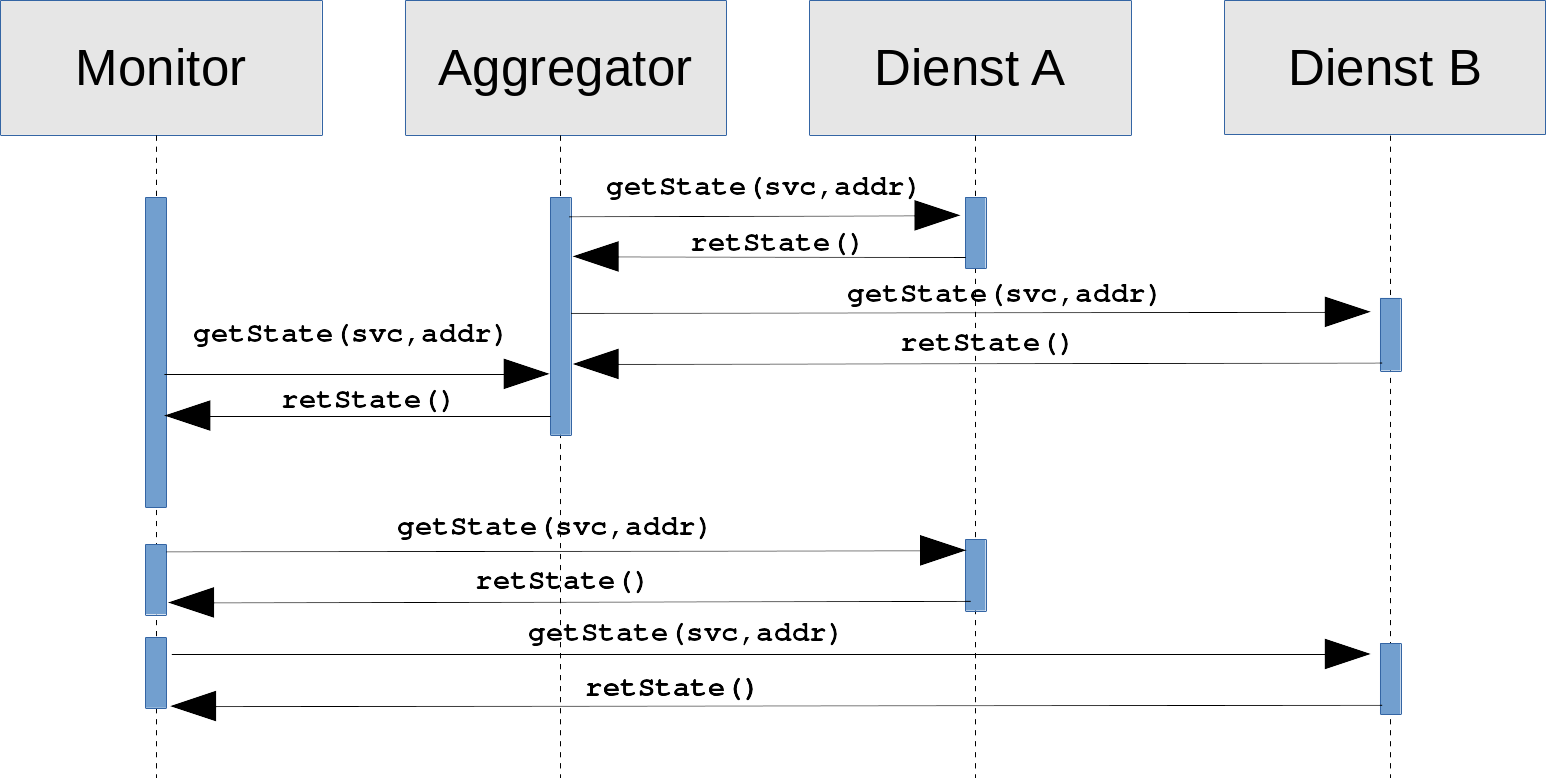
\includegraphics[scale=0.25]{img/sequence_uml_active_trans.png}

\end{frame}


\begin{frame}
\frametitle{Passive Überwachung}
\framesubtitle{Beispiel Sequenzdiagramm}

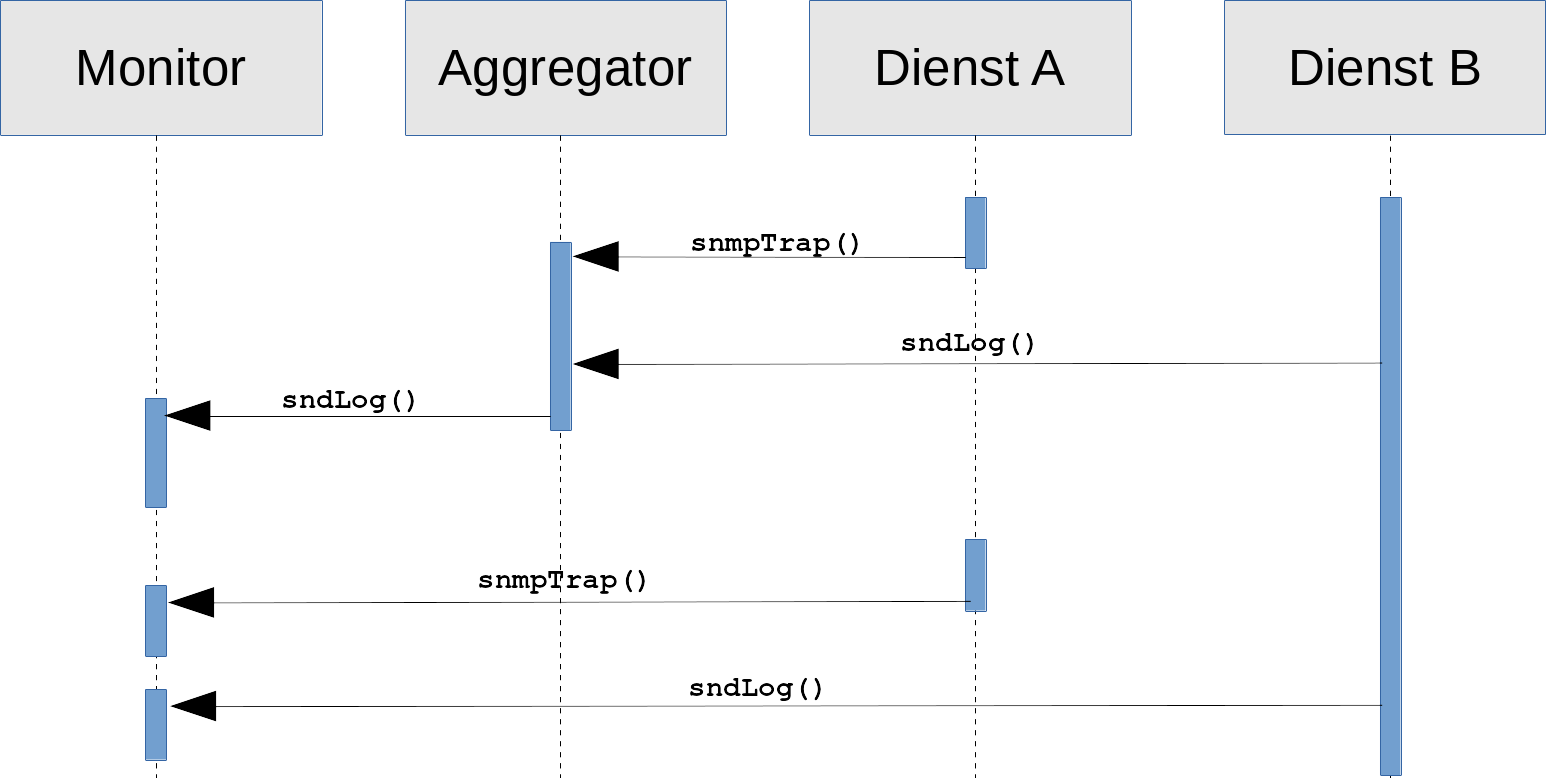
\includegraphics[scale=0.25]{img/sequence_uml_passive_trans.png}

\end{frame}
